\documentclass[UTF8]{ctexart}
\usepackage{graphicx}
\title{实验二:单周期CPU}
\author{陈子轩 516030910545}
\date{\today}

\begin{document}
\maketitle
\section{实验目的和实验步骤}
请参考实验指导书
\section{实验设计思路}
\subsection{整体工程的构建}
由于已经给出了90\%的源代码,所以整体工程的构建比较简单,顶层由CPU, 数据内存和指令内存构成。CPU又由cu(control unit), alu, regfile以及各种多路选择器构成。指令内存由封装好的指令rom构成。这里我们需要考虑的关键在于数据内存(data memory).
\subsection{数据内存的构建}
\begin{figure}
	\centering
	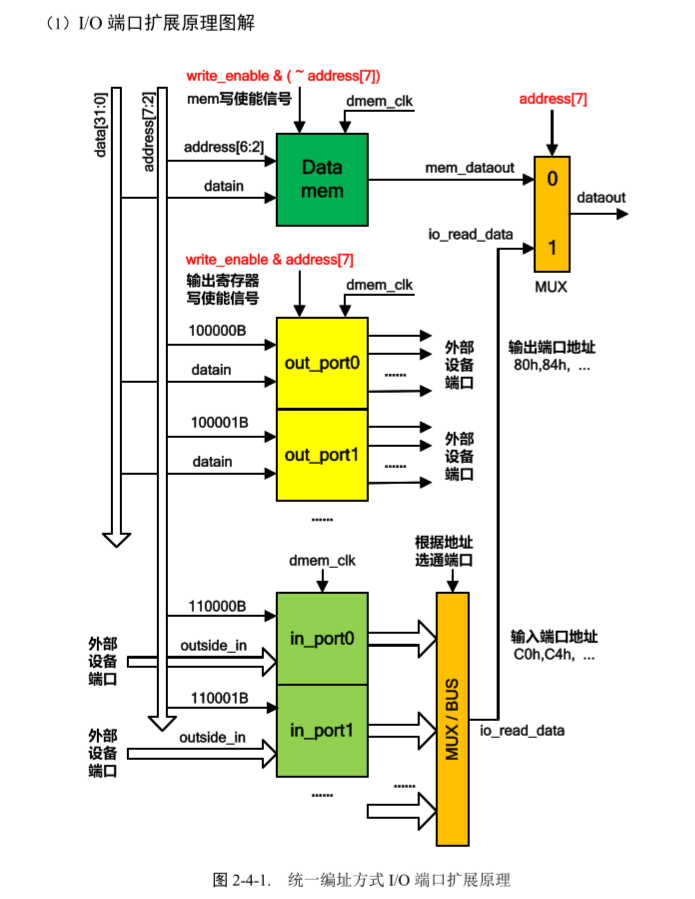
\includegraphics{uioaddr.PNG}
	\caption{统一编址方式}
\end{figure}
由于需要通过FPGA与我们设计的CPU进行交互,所以我们需要将从FPGA中输入的内容转移到CPU中,这里我们采用io和内存的统一编码方式,通过设计一系列的接口(in\_port, out\_port)来模拟内存的输入输出,在按照一定的方式和FPGA进行对接,从而完成交互,如图一所示。
\paragraph{}

在设计中我采用了3个in\_port接口对应操作数1(operand1, $sw[3:0]$),操作数2(operand2, $sw[7:4]$),和操作类型(type of operation, $sw[9:8]$)。采用了三个out\_port接口对应操作数1(operand1, hex0, hex1),操作数2(operand2, hex2, hex3)和操作结果(result, hex4, hex5)。实际采用了四种算术运算(add, sub, and, or)进行测试。

\subsection{FPGA适配器的构建}
上述情况中我们需要将各种in\_port和out\_port对应到我们的FPGA上。
\newline
\begin{tabular}{|l|l|} %l(left)居左显示 r(right)居右显示 c居中显示
	\hline
	in\_port0 & sw[3:0] \\
	\hline
	in\_port1 & sw[7:4] \\
    \hline
    in\_port2 & sw[9:8] \\
    \hline
    out\_port0 & hex0, hex1 \\
    \hline
    out\_port1 & hex2, hex3 \\
    \hline
    out\_port2 & hex4, hex5 \\
    \hline
\end{tabular}

\section{源代码}
下面提供一些自己设计的代码,实验提供的源码则作忽略
\begin{verbatim}

module sc_datamem (addr, datain, dataout, we, clock, mem_clk, dmem_clk,
                    resetn, mem_dataout, io_read_data, in_port0, in_port1, in_port2,
                    out_port0, out_port1, out_port2);
    //数据内存,采用io和memory的统一编码
    input [31:0]   addr;
    input [31:0]   datain;
    input          resetn;
    input          we, clock, mem_clk;
    input [31:0]   in_port0, in_port1, in_port2;

    output [31:0]  dataout;
    output         dmem_clk;
    output [31:0]  out_port0, out_port1, out_port2;
    output [31:0]  mem_dataout;
    output [31:0]  io_read_data;

    wire           dmem_clk;
    wire           write_enable;
    wire 				writ_datamem_enable, write_io_output_reg_enable;
    wire[31:0]     mem_dataout;
    reg[31:0] 		out_port0, out_port1, out_port2, io_read_data;

    assign         write_enable = we & ~clock;
    assign         dmem_clk = mem_clk & ( ~ clock);
    assign         writ_datamem_enable = write_enable & (~addr[7]);
    assign         write_io_output_reg_enable = write_enable & (addr[7]);

    mux2x32 mem_io_dataout_mux(mem_dataout, io_read_data, addr[7], dataout);

    lpm_ram_dq_dram  dram(addr[6:2],dmem_clk,datain,write_enable, mem_dataout );

    always @(posedge mem_clk)
        begin
            if (addr[7:2] == 6'b100000) //128 对应操作数1
            io_read_data <= in_port0;
            else if (addr[7:2] == 6'b100001) //132 对应操作数2
            io_read_data <= in_port1;
            else if (addr[7:2] == 6'b100010) //136 对应操作类型
            io_read_data <= in_port2;
            else
            io_read_data <= 0;

            out_port0 <= in_port0;
            out_port1 <= in_port1;
            if(addr[7:2] == 6'b100011) //144对应运算结果
            out_port2 <= datain;
        end

endmodule

module in_port_adapter(sw, in_port0, in_port1, in_port2);

    input [9:0] sw;
    output [31:0] in_port0, in_port1, in_port2;

    assign in_port0 = {28'b0, sw[3:0]};
    assign in_port1 = {28'b0, sw[7:4]};
    assign in_port2 = {30'b0, sw[9:8]};

endmodule

module out_port_adapter(hex0, hex1, hex2, hex3, hex4, hex5, out_port0, out_port1, out_port2);

    input [31:0] out_port0, out_port1, out_port2;

    output [6:0] hex0, hex1, hex2, hex3, hex4, hex5;

    wire [3:0] a0, a1, b0, b1, c0, c1;
    assign a0 = out_port0 % 10;
    assign a1 = out_port0 / 10;
    assign b0 = out_port1 % 10;
    assign b1 = out_port1 / 10;
    assign c0 = out_port2 % 10;
    assign c1 = out_port2 / 10;

    sevenseg h0(a0, hex0);
    sevenseg h1(a1, hex1);
    sevenseg h2(b0, hex2);
    sevenseg h3(b1, hex3);
    sevenseg h4(c0, hex4);
    sevenseg h5(c1, hex5);

endmodule


//4bit 的BCD码至 7 段 LED数码管译码器模块
module sevenseg ( theta, ledsegments);
    input [3:0] theta;
    output [6:0] ledsegments;
    reg [6:0] ledsegments;
    always @ (*)
        case(theta)
        // //gfe_dcba 654_3210
        0: ledsegments = 7'b100_0000;				// DE2C板上的数码管为共阳极接法
        1: ledsegments = 7'b111_1001;
        2: ledsegments = 7'b010_0100;
        3: ledsegments = 7'b011_0000;
        4: ledsegments = 7'b001_1001;
        5: ledsegments = 7'b001_0010;
        6: ledsegments = 7'b000_0010;
        7: ledsegments = 7'b111_1000;
        8: ledsegments = 7'b000_0000;
        9: ledsegments = 7'b001_0000;
        default: ledsegments = 7'b111_1111; 	// 其它值时全灭
        endcase
endmodule

module sc_cu (op, func, z, wmem, wreg, regrt, m2reg, aluc, shift,
    aluimm, pcsource, jal, sext);
    input  [5:0] op,func;
    input        z;
    output       wreg,regrt,jal,m2reg,shift,aluimm,sext,wmem;
    output [3:0] aluc;
    output [1:0] pcsource;
    wire r_type = ~|op;
    wire i_add = r_type & func[5] & ~func[4] & ~func[3] &
    ~func[2] & ~func[1] & ~func[0];          //100000
    wire i_sub = r_type & func[5] & ~func[4] & ~func[3] &
    ~func[2] &  func[1] & ~func[0];          //100010

    //  please complete the deleted code.

    wire i_and = r_type & func[5] & ~func[4] & ~func[3] & func[2] & ~func[1] & ~func[0]; // 100100
    wire i_or  = r_type & func[5] & ~func[4] & ~func[3] & func[2] & ~func[1] & func[0]; // 100101

    wire i_xor = r_type & func[5] & ~func[4] & ~func[3] & func[2] & func[1] & ~func[0] ; // 100110
    wire i_sll = r_type & ~func[5] & ~func[4] & ~func[3] & ~func[2] & ~func[1] & ~func[0]; // 000000
    wire i_srl = r_type & ~func[5] & ~func[4] & ~func[3] & ~func[2] & func[1] & ~func[0] ; // 000001
    wire i_sra = r_type & ~func[5] & ~func[4] & ~func[3] & ~func[2] & func[1] & func[0]; // 000011
    wire i_jr  = r_type & ~func[5] & ~func[4] & func[3] & ~func[2] & ~func[1] & ~func[0]; // 001000

    wire i_addi = ~op[5] & ~op[4] &  op[3] & ~op[2] & ~op[1] & ~op[0]; //001000
    wire i_andi = ~op[5] & ~op[4] &  op[3] &  op[2] & ~op[1] & ~op[0]; //001100

    wire i_ori  = ~op[5] & ~op[4] & op[3] & op[2] & ~op[1] & op[0] ; // 001101
    wire i_xori = ~op[5] & ~op[4] & op[3] & op[2] & op[1] & ~op[0] ; // 001110
    wire i_lw   = op[5] & ~op[4] & ~op[3] & ~op[2] & op[1] & op[0] ; // 100011
    wire i_sw   = op[5] & ~op[4] & op[3] & ~op[2] & op[1] & op[0] ; // 101011
    wire i_beq  = ~op[5] & ~op[4] & ~op[3] & op[2] & ~op[1] & ~op[0]  ; // 000100
    wire i_bne  = ~op[5] & ~op[4] & ~op[3] & op[2] & ~op[1] & op[0] ; //000101
    wire i_lui  = ~op[5] & ~op[4] & op[3] & op[2] & op[1] & op[0] ; // 001111
    wire i_j    = ~op[5] & ~op[4] & ~op[3] & ~op[2] & op[1] & ~op[0] ; // 000010
    wire i_jal  = ~op[5] & ~op[4] & ~op[3] & ~op[2] & op[1] & op[0] ; // 000011


    assign pcsource[1] = i_jr | i_j | i_jal;
    assign pcsource[0] = ( i_beq & z ) | (i_bne & ~z) | i_j | i_jal ;

    assign wreg = i_add | i_sub | i_and | i_or   | i_xor  |
    i_sll | i_srl | i_sra | i_addi | i_andi |
    i_ori | i_xori | i_lw | i_lui  | i_jal;

    assign aluc[3] = i_sra;
    assign aluc[2] = i_sub | i_or | i_srl | i_sra | i_ori | i_lui | i_beq | i_bne;
    assign aluc[1] = i_xor | i_sll | i_srl | i_sra | i_xori | i_lui ;
    assign aluc[0] = i_and | i_or | i_sll | i_srl | i_sra | i_andi | i_ori;
    assign shift   = i_sll | i_srl | i_sra ;

    assign aluimm  = i_addi | i_andi | i_ori | i_xori | i_lw | i_sw | i_lui;
    assign sext    = 1;
    assign wmem    = i_sw;
    assign m2reg   = i_lw;
    assign regrt   = i_addi | i_andi | i_ori | i_xori | i_lw | i_sw | i_lui;
    assign jal     = i_jal;

endmodule

module alu (a,b,aluc,s,z);
    input [31:0] a,b;
    input [3:0] aluc;
    output [31:0] s;
    output        z;
    reg [31:0] s;
    reg        z;
    always @ (a or b or aluc)
        begin                                   // event
            casex (aluc)
                4'bx000: s = a + b;              //x000 ADD
                4'bx100: s = a - b;              //x100 SUB
                4'bx001: s = a & b;			  //x001 AND
                4'bx101: s = a | b;              //x101 OR
                4'bx010: s = a ^ b;              //x010 XOR
                4'bx110: s = a << 16;		      //x110 LUI: imm << 16bit
                4'b0011: s = b << a;             //0011 SLL: rd <- (rt << sa)
                4'b0111: s = b >> a;             //0111 SRL: rd <- (rt >> sa) (logical)
                4'b1111: s = $signed(b) >>> a;   //1111 SRA: rd <- (rt >> sa) (arithmetic)
                default: s = 0;
            endcase
            if (s == 0 )  z = 1;
            else z = 0;
        end
endmodule
\end{verbatim}
\end{document}